\section{Methodischer Ansatz}\label{sec:methodology}

\subsection{Use Case}

Der betrachtete Use Case beschreibt einen mittelgroßen Wiener Parkhausbetreiber mit \mbox{200--500} Stellplätzen in einer innerstädtischen Lage. Der Betreiber sieht sich mit schwankender Auslastung, wachsendem Wettbewerbsdruck durch alternative Mobilitätsangebote und unsicheren Pendlerströmen aus dem Umland konfrontiert \citep{wangEconomicsSmartParking2025}. Aus betrieblicher Sicht stellt sich daher die Frage, ob eine Investition in ein \ac{sps} wirtschaftlich gerechtfertigt werden kann.

Klassische Parkleitsysteme zeigen freie Stellplätze nur statisch oder lokal an einer Anzeigetafel an \citep{stadtwienParkleitsystemFuerWien2026}. Ein \ac{iot}-basiertes \ac{sps} könnte dem gegenüber Echtzeit-Belegungsdaten in Navigationssysteme und Apps einspielen, dynamische Tarife unterstützen und Daten zur Auslastung systematisch erfassen \citep{sarkerSmartParkingSystem2020}. Damit verschiebt sich die Diskussion von der reinen Machbarkeit hin zur Frage nach belastbaren Kennzahlen für die Investitionsentscheidung.

Drive \& Decide adressiert genau diese Lücke. Der Use Case definiert den Betreiber als Entscheidungsträger und die Investition in Sensorik, Konnektivität und Cloud-Backend als zu bewertende Maßnahme. Endnutzer:innen treten als indirekte Akteure auf, deren Verhalten den Nutzen des Systems beeinflusst, jedoch nicht selbst Gegenstand der Bewertung ist.

\subsection{Technische Beschreibung des Versuchsaufbaus}

Abbildung \ref{fig:architecture} zeigt die Systemarchitektur im Überblick und dient als Orientierung für die folgenden Absätze. Der Versuchsaufbau ist bewusst zweigeteilt, um zwei unterschiedliche Erkenntnisinteressen abzudecken. Ein physischer Prototyp dient der realistischen Erfassung von Sensor- und Kommunikationsverhalten, während ein virtueller Prototyp die Skalierung auf eine ganze Parkgarage erlaubt. Diese Kombination ermöglicht es, sowohl reale Messwerte als auch lastabhängige Cloud-Kosten zu erheben.

Der physische Prototyp besteht aus einem 3D-gedruckten Modell einer Parkgarage mit mehreren Stellplätzen, die mit Matchbox-Fahrzeugen belegt werden. Pro Stellplatz wird ein Belegungssensor verbaut, etwa ein \ac{ir}- oder \ac{tof}-Sensor, da diese Bauarten kostengünstig, kompakt und gut für eingebettete Anwendungen verfügbar sind \citep{perkovicSmartParkingSensors2020}. Die Sensoren werden über einen Mikrocontroller, beispielsweise einen ESP32, ausgelesen und die Belegungsereignisse via \ac{mqtt} an die Cloud übertragen.

Der virtuelle Prototyp simuliert eine Parkgarage mit einer größeren Anzahl an Stellplätzen sowie ein Ampelsystem an der Einfahrt, das Belegungszustände aggregiert anzeigt. Belegungsereignisse werden in einem definierten Lastprofil generiert und über denselben \ac{mqtt}-Pfad in die Cloud geschickt wie beim physischen Modell. Auf diese Weise lassen sich realitätsnahe Lastszenarien für mehrere hundert Stellplätze durchspielen, ohne entsprechende Hardware physisch verbauen zu müssen.

Das Backend folgt einer serverlosen Architektur auf \ac{aws}. \ac{aws} \ac{iot} Core übernimmt die Geräteanbindung und das Routing der \ac{mqtt}-Nachrichten, \ac{aws} Lambda verarbeitet eingehende Events ereignisgetrieben und Amazon DynamoDB speichert den aktuellen Belegungsstatus. Dieser Aufbau ist typisch für aktuelle \ac{iot}-getriebene \acp{sps} und vermeidet permanent betriebene Server, was für die spätere Kostenmodellierung von zentraler Bedeutung ist \citep{alaanzyRealTimeSmart2025,alamSurveyIoTDriven2023}.

\begin{figure}[!ht]
    \centering
    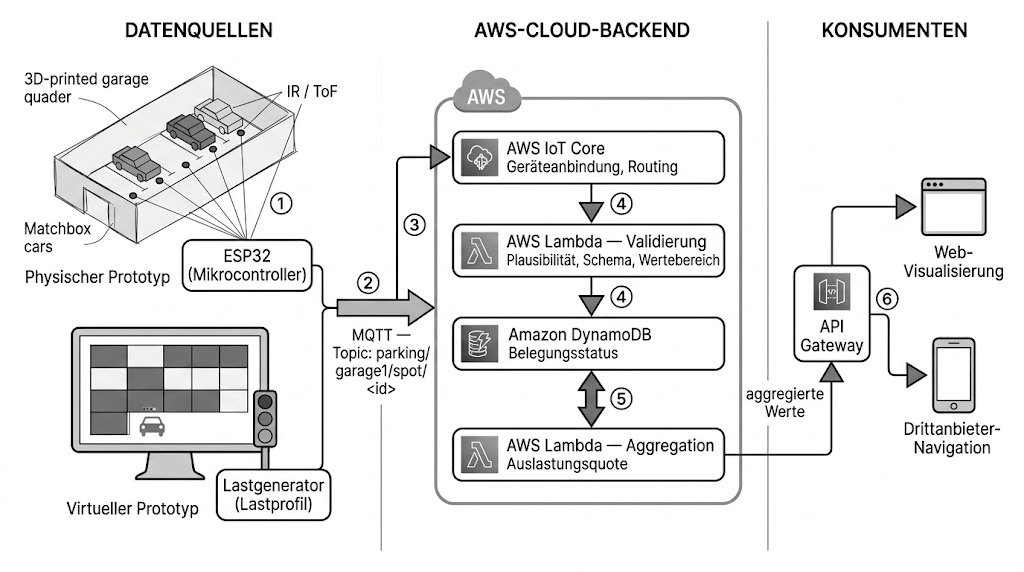
\includegraphics[width=\linewidth]{fig/architecture.jpg}
    \caption{Systemarchitektur von Drive \& Decide}
    \Description[Systemarchitektur]{Systemarchitektur von Drive \& Decide}
    \label{fig:architecture}
\end{figure}
\FloatBarrier

\subsection{Datenfluss und Verarbeitung}

Der in Abbildung \ref{fig:architecture} skizzierte Datenfluss von der Sensorebene bis zur Ausgabeschnittstelle lässt sich in sechs klar abgegrenzte Schritte gliedern:
(1) ein Sensor erkennt einen Wechsel des Belegungsstatus eines einzelnen Stellplatzes,
(2) der Mikrocontroller formt daraus eine \ac{mqtt}-Nachricht mit Sensor-ID, Stellplatz-ID, Zeitstempel, Rohmesswert und abgeleitetem Status \citep{sarkerSmartParkingSystem2020},
(3) die Nachricht wird auf einem strukturierten Topic, etwa \texttt{parking/garage1/spot/123}, gegenüber \ac{aws} \ac{iot} Core veröffentlicht,
(4) eine \ac{iot}-Rule routet die Nachricht an eine Lambda-Funktion, die Plausibilität, Schemata und Wertebereiche prüft und den validierten Status in DynamoDB schreibt,
(5) bei Bedarf wird eine Aggregations-Lambda zur Berechnung der aktuellen Auslastungsquote angestoßen und
(6) eine \ac{api} Gateway-Schnittstelle stellt die aggregierten Werte für externe Konsumenten bereit, etwa für eine schlanke Web-Visualisierung oder Drittanbieter-Navigationssysteme.

Damit ist der Datenfluss in jedem Schritt mess- und kostenseitig instrumentierbar. Dieser durchgehend ereignisgetriebene Aufbau ist eine Voraussetzung dafür, dass nutzungsabhängige Cloud-Kosten belastbar erfasst werden können. Die so gewonnenen Verbrauchsdaten gehen direkt als Eingangsgrößen in das nachfolgende Kosten-Nutzen-Modell ein.

\subsection{Kosten-Nutzen-Analyse}

Das Kosten-Nutzen-Modell ist das Herzstück des methodischen Ansatzes und wird aus Sicht des Betreibers aufgebaut. Es stellt einmaligen Investitions- und laufenden Betriebskosten den erwarteten zusätzlichen Erlös einer besseren Auslastung gegenüber. Bewertungshorizont ist ein Zeitraum von fünf Jahren, da dieser typischen Abschreibungszeiträumen für IT- und Sensor-Infrastruktur entspricht.

Auf der Kostenseite werden \ac{capex} und \ac{opex} getrennt erfasst:
\begin{itemize}
    \item \textbf{\ac{capex}:} Sensoren je Stellplatz, Mikrocontroller, Verkabelung, Installation sowie initiale Cloud-Konfiguration
    \item \textbf{\ac{opex}:} nutzungsabhängige \ac{aws}-Kosten für \ac{iot} Core, Lambda, DynamoDB, Datentransfer und Speicher, ergänzt um Wartung, Sensoraustausch und Stromverbrauch
\end{itemize}

Auf der Nutzenseite werden vier Wirkungspfade modelliert:
\begin{enumerate}
    \item Erhöhte Auslastung durch verlässlichere Auffindbarkeit freier Stellplätze in Apps und Navigationssystemen \citep{alaanzyRealTimeSmart2025}
    \item Zusätzliche Erlöspotenziale durch dynamische Preisgestaltung in Stoßzeiten \citep{hassineDynamicPricingRoute2024,sarkerSmartParkingSystem2020}
    \item Reduzierte Fehlfahrten und damit indirekte Reputationseffekte
    \item Potenzieller Zusatznutzen aus der Verwertung anonymisierter Auslastungsdaten, beispielsweise gegenüber Stadt oder Mobilitätsdiensten \citep{wangEconomicsSmartParking2025}
\end{enumerate}

Die wirtschaftliche Sinnhaftigkeit wird anhand von vier Kennzahlen beurteilt:
\begin{enumerate}
    \item \ac{tco} über fünf Jahre, gebildet aus \ac{capex} und kumulierten \ac{opex}
    \item \ac{roi} im Verhältnis zum geschätzten Mehrerlös
    \item Amortisationsdauer in Monaten
    \item Break-Even-Punkt, also jene zusätzliche Auslastungssteigerung in Prozentpunkten, ab der das System sich trägt
\end{enumerate}

Die Datenerhebung kombiniert drei Quellen. Sensor- und Hardware-Stückkosten werden aus aktuellen Markt- und Herstellerangaben abgeleitet, \ac{aws}-Kosten werden über den \ac{aws} Pricing Calculator ermittelt und Nutzenparameter wie erwartbare Auslastungssteigerung oder Preiselastizität werden aus der einschlägigen Literatur übernommen \citep{wangEconomicsSmartParking2025,sarkerSmartParkingSystem2020}. Eine abschließende Sensitivitätsanalyse variiert Stellplatzanzahl, Sensor-Stückkosten und unterstellte Auslastungssteigerung, um die Robustheit der Aussage gegenüber Modellannahmen zu prüfen.

\subsection{Abgrenzung}

Die Arbeit verspricht keine flächendeckende Smart-Parking-Lösung für Wien, sondern einen nachvollziehbaren Bewertungsrahmen für einen einzelnen Betreiber. Es wird kein vergleichender Sensor-Benchmark verschiedener Technologien durchgeführt, da bestehende Übersichtsstudien diese Frage bereits adressieren \citep{perkovicSmartParkingSensors2020,fahimSmartParkingSystems2021}. Ebenso wird keine Endnutzerstudie zur App-Akzeptanz vorgenommen. Gesellschaftliche Effekte wie Verkehrssicherheit werden qualitativ eingeordnet.

Modellannahmen wie Garagengröße, angenommene Auslastung, Sensor-Lebensdauer oder \ac{aws}-Tarifmodell werden offen dokumentiert, sodass das Modell für andere Profile von Betreibern reproduzierbar bleibt. Verschieben sich Marktbedingungen oder Hardwarepreise im Zeitverlauf, lassen sich die betroffenen Parameter gezielt anpassen, ohne den methodischen Rahmen zu verändern. Der wissenschaftliche Beitrag liegt damit nicht in einer einzelnen Komponente, sondern in der methodischen Verbindung aus realitätsnahem Versuchsaufbau, vollständig instrumentiertem Cloud-Datenfluss und einem darauf aufbauenden Kosten-Nutzen-Modell aus Sicht des Betreibers.
